  \chapter{Výběr bezdrátové technologue pro senzorovou síť}
Navržená senzorová síť je napojena na infrastrukturu zavedeného přístupového systému v budově zákazníka s dosahem po celé budově a jejím okolí. Takto navržená síť umožní v těchto prostorách snímání dat z desítek senzorů.
Mezi hlavní kritéria pro vybranou bezdrátovou technologii patří nízká spotřeba energie koncových zařízení, nízká cena, jednoduchost implementace a možnost připojení koncových zařízení třetích stran.
Pro jednoduchost implementace vybraná bezdrátová technologie tedy používá bezlicenční pásmo ISM. 

\section{Kandidátní bezdrátové technlogie}
Níže jsou popsány dostupné bezdrátové technologie vyhovující stanoveným kritériím pro tento projekt.

\begin{table}[]
  \begin{tabular}{|p{1.5cm}||p{2cm}|p{2cm}|p{2cm}|p{2cm}|p{2cm}|}
  \hline
  Technology    & topology options                & frequency bands  & range                                           & price per one transciever & availability of devices on the market \\ \hline \hline
  IQRF           & mesh, star                      & 868 MHz (Europe) & 10-100 m (in building), 100-1000 m (open space) & 15 – 20 \$                & very low                              \\ \hline
  wireless M-bus & star                            & 868M, 433M, 169M & 500 m (868 MHz), 2000 m (169 MHz)               & 25 – 30 \$                & low                                   \\ \hline
  ZigBee         & mesh, star                      & 2.4 GHz          & 100 m (open space)                              & 8 – 30 \$                 & high                                  \\ \hline
  BLE            & Point-to-Point, Broadcast, Mesh & 2.4 GHz          & 100 m (open space)                              & 5 – 20 \$                 & high                                  \\ \hline
  LoRa           & star                            & 868 MHz (Europe) & 15-22 km suburban, 3-8 km urban                 & 5 – 50 \$                 & medium                                \\ \hline
  Z-Wave         & mesh                            & 868 MHz (Europe) & 100 m in (open space), 30 m (in building)       & 10 – 50 \$                & high                                  \\ \hline
  Thread         & mesh                            & 2.4 GHz          & 100 m (open space)                              & 30 – 50 \$                & low                                   \\ \hline
  \end{tabular}
\end{table}

\subsection{IQRF}
IQRF je subGHz bezdrqátová technologie vyvinuta IQRF aliancí \cite{iqrf_alliance}, která je jediným výrobcem IQRF transceiveru \cite{iqrf_transceivers} za cenu v rozsahu \$15-20 za kus a k tomu poskytuje nástroje jako je SDK \cite{iqrf_sdk} a IDE \cite{iqrf_ide}. Z hlediska kriérií pro tento projekt je u této technologie nevýhodou nízký počet zařízení třetích stran dostupných na trhu. 
Většinou je tato technologie použita pro realizaci uživatelsé sítě, kde gateway je použita jedna z dostupných od IQRF aliance a koncová zařízení sítě jsou vytvořena vývojáři s použitím transceiverů od IQRF aliance
\cite{paper_iqrf}.


\section{Wireless M-bus}
\textit{"Wireless Meter Bus has its origins within the Meter-Bus standards. This is a field bus standard aimed at applications for collecting meter data for gas, electricity, water, etc."} \cite{5}
It supports a few application modes for differing applications.
\begin{itemize}
  \item S1  Unidirectional, data are transmitted only a several times a day.
  \item S2	Bidirectional version of S1.
  \item	T1	Unidirectional transmission of data with a period of a few seconds of minutes.
  \item T2	Bidirectional version of T1.
  \item C1	Unidirectional transmission of bigger amount of data.
  \item C2	Bidirectional version of C1.
\end{itemize}
Usually one M-bus device support only a few of these application modes \cite{5} \cite{6} \cite{7} \cite{8}.


\section{Zigbee}
Zigbee, developed by zigbee alliance is usually used for mesh sensor networks because of its short range. This technology is standardized since 2003, so there is many available nodes at the market by now \cite{10} \cite{11} \cite{12}.

\section{BLE}
Bluetooth has the big advantage, taht it's built in almost every mobile phone, tablet or laptop so there are more options to control the network. The Bluetooth 4.0+ also called BLE (Bluetooth Low Energy) aims to low power wireless sensor networks.
It can be used for point-to-point, broadcast or mesh network topology \cite{13} \cite{14} \cite{15} \cite{16}.


\section{LoRa}
The name LoRa stands for "Long Range" wireless communication with low data rate and power consumption. The protocol enables to modify SF which affects the communication range and data rate. The \ref{fig:loraSF} shows this dependence.

\begin{figure}[!h]
    \centering
    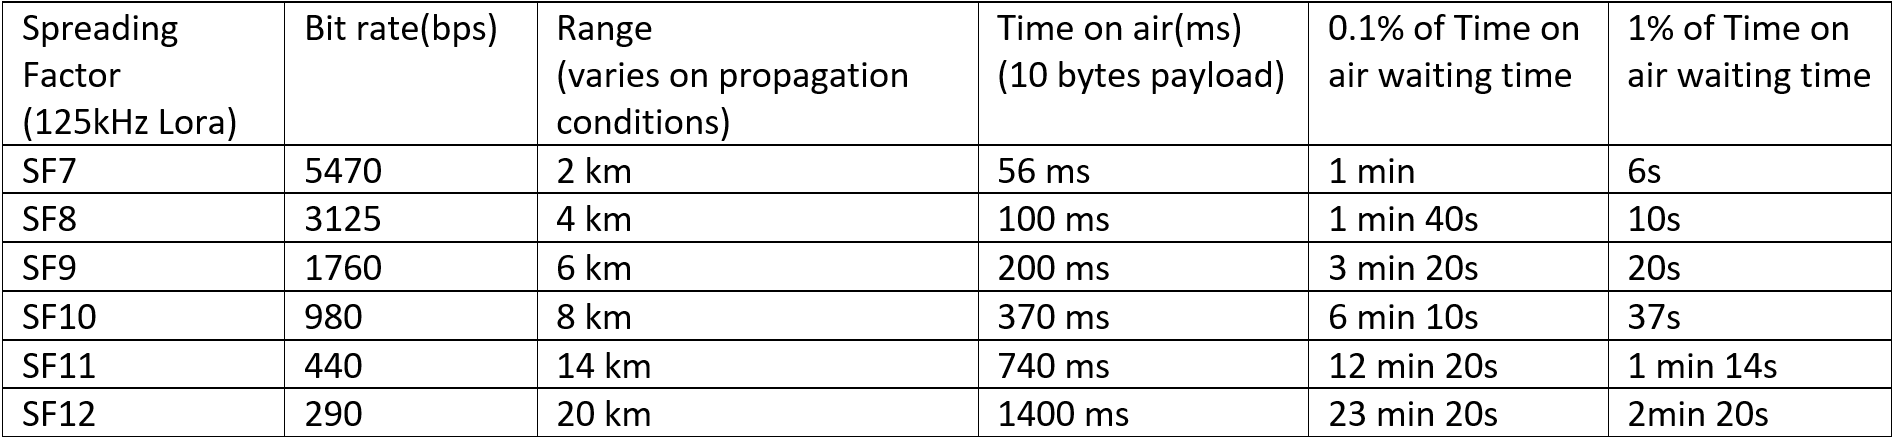
\includegraphics[width=1\textwidth]{spreading_factor_lorawan_2017-07-29}
    \caption{LoRa spread factor options \cite{24}}
    \label{fig:loraSF}
\end{figure}

This technology is very attractive for its long range capability and easy to connect nodes. It's complicated to build a full-capacity gateway which is capable of receiving packets at all frequency channels and SF in parallel. The transceiver for this application costs about \$130. Although it's also possible to build single-channel gateway which is way too cheaper, but it can receive packets at only one frequency channel and SF at once \cite{17} \cite{18} \cite{19} \cite{20} \cite{21} \cite{22} \cite{23} \cite{24}.


\section{Z-Wawe}
Z-Wave is intended for wireless connectivity for all possible smart home products, controlled by PC, phone, voice, etc. It's based on mesh network topology so every non-battery powered device works as a router to enhance the network range so the more devices are connected in one network, the stronger the network is \cite{27} \cite{28}.


\section{Thread}
This technology based on IPv6 was developed for home network controlled by smartphone, tablet or PC \cite{29} \cite{30} \cite{31}.








\subsection{Wireless Sensor Network Design}
Wireless sensor network design is based on a popular IoT technology LoRa, which is a LPWAN technology using ISM band, 433 MHz, 868 MHz and 915 MHz (depends on the region) and communicates on multiple frequency channels and uses multiple data rates \cite{LoRaWAN Evaluation for IoT Communications}.
The LoRaWAN is an open standard network protocol and system architecture specified by \cite{LoRaWAN specification} and creates a media access control (MAC) layer on the top of the LoRa physical layer, secured by AES-128 encryption.
The LoRaWAN nodes communicate directly with the LoRaWAN gateway \cite{Internet of Things (IoT) using LoRa technology}.


